\documentclass[12pt]{article}
\usepackage{amsmath}
\usepackage{fancyhdr}
\usepackage{tikz}
\usepackage{pgfplots}
\usetikzlibrary{shapes,backgrounds}
\usepackage[margin=1in]{geometry}

\pagestyle{fancy}
\lhead{CSCI 6550}
\chead{\textbf{Week 1 Assignment Report}}
\rhead{Eric Miller}

\begin{document}
\subsection*{Introduction}


\subsection*{Results}
\subsubsection*{Minimax vs. Minimax}
\begin{center}
    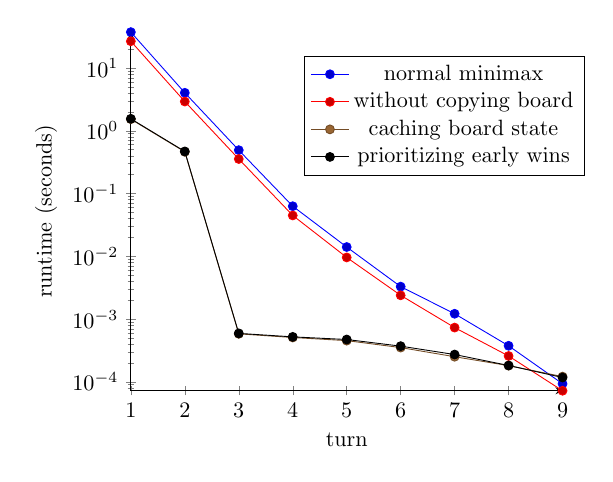
\begin{tikzpicture}[scale=.8]
        \begin{axis}[
            legend style={at={(.4,.6)},anchor=south west},
            axis lines = left,
            xlabel = turn,
            xtick = {0, 1, 2, 3, 4, 5, 6, 7, 8, 9},
            ymode = log,
            ylabel = runtime (seconds),
        ]
        \addplot+[
            mark=*,
        ] plot coordinates{
            (1,37.328725)
            (2,4.028346)
            (3,0.490918)
            (4,0.062810)
            (5,0.014050)
            (6,0.003286)
            (7,0.001214)
            (8,0.000375)
            (9,0.000093)
        };
        \addlegendentry{normal minimax}
        \addplot+[
            mark=*,
        ] plot coordinates{
            (1,26.668035)
            (2,2.922236)
            (3,0.354789)
            (4,0.044750)
            (5,0.009588)
            (6,0.002387)
            (7,0.000731)
            (8,0.000258)
            (9,0.000072)
        };
        \addlegendentry{without copying board}
        \addplot+[
            mark=*,
        ] plot coordinates{
            (1,1.530653)
            (2,0.462433)
            (3,0.000581)
            (4,0.000508)
            (5,0.000453)
            (6,0.000351)
            (7,0.000251)
            (8,0.000181)
            (9,0.000121)
        };
        \addlegendentry{caching board state}
        \addplot+[
            mark=*,
        ] plot coordinates{
            (1,1.551102)
            (2,0.468198)
            (3,0.000591)
            (4,0.000520)
            (5,0.000472)
            (6,0.000370)
            (7,0.000272)
            (8,0.000182)
            (9,0.000117)
        };
        \addlegendentry{prioritizing early wins}
        
        \end{axis}
    \end{tikzpicture} 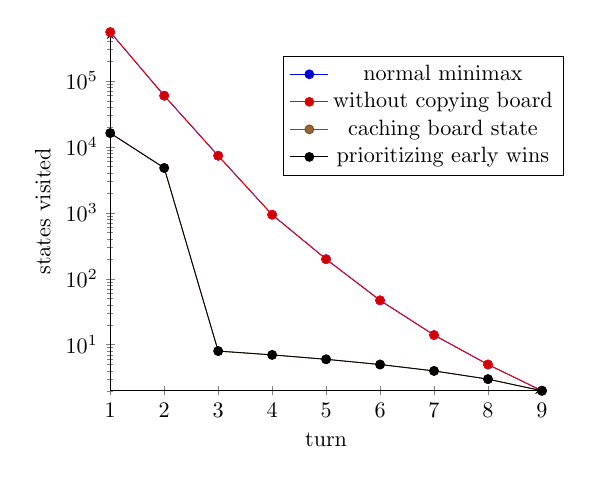
\begin{tikzpicture}[scale=.8]
        \begin{axis}[
            legend style={at={(.4,.6)},anchor=south west},
            axis lines = left,
            xlabel = turn,
            xtick = {0, 1, 2, 3, 4, 5, 6, 7, 8, 9},
            ymode = log,
            ylabel = states visited,
        ]
        \addplot+[
            mark=*,
        ] plot coordinates{
            (1,549946)
            (2,59705)
            (3,7332)
            (4,935)
            (5,198)
            (6,47)
            (7,14)
            (8,5)
            (9,2)
        };
        \addlegendentry{normal minimax}
        \addplot+[
            mark=*,
        ] plot coordinates{
            (1,549946)
            (2,59705)
            (3,7332)
            (4,935)
            (5,198)
            (6,47)
            (7,14)
            (8,5)
            (9,2)
        };
        \addlegendentry{without copying board}
        \addplot+[
            mark=*,
        ] plot coordinates{
            (1,16168)
            (2,4792)
            (3,8)
            (4,7)
            (5,6)
            (6,5)
            (7,4)
            (8,3)
            (9,2)
        };
        \addlegendentry{caching board state}
        \addplot+[
            mark=*,
        ] plot coordinates{
            (1,16168)
            (2,4792)
            (3,8)
            (4,7)
            (5,6)
            (6,5)
            (7,4)
            (8,3)
            (9,2)
        };
        \addlegendentry{prioritizing early wins}
        
        \end{axis}
    \end{tikzpicture}
\end{center}

\subsubsection*{Minimax vs. Random}
\begin{center}
    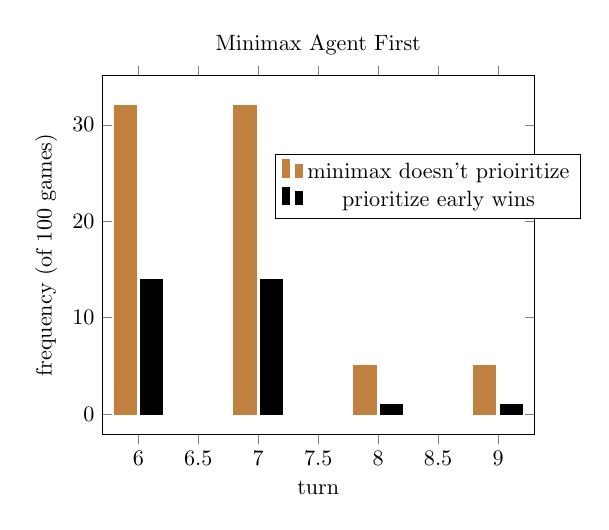
\begin{tikzpicture}[scale=.8]
        \begin{axis}[
            legend style={at={(.4,.6)},anchor=south west},
            ybar,
            xlabel = turn,
            ylabel = frequency (of 100 games),
            title= Minimax Agent First
        ]
        %Below the red parabola is defined
        \addplot+[
            color = brown
        ]
        plot coordinates{
            (6,32)
            (7,32)
            (8,5)
            (9,5)
        };
        \addlegendentry{minimax doesn't prioiritize}

        \addplot+[
            color = black
        ]
        plot coordinates{
            (6,14)
            (7,14)
            (8,1)
            (9,1)
        };
        \addlegendentry{prioritize early wins}

        \end{axis}
    \end{tikzpicture}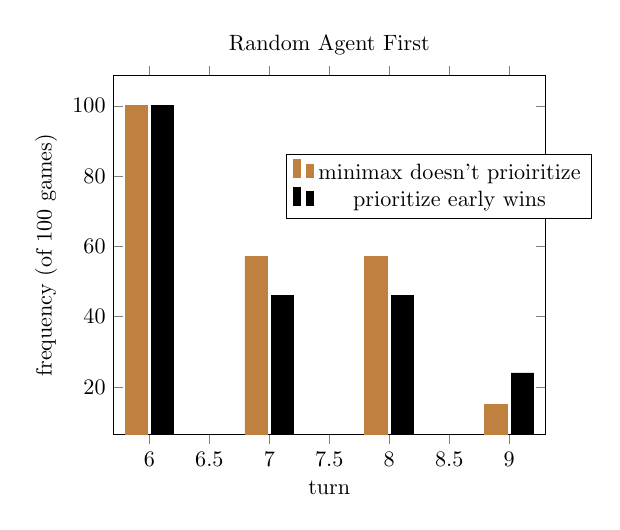
\begin{tikzpicture}[scale=.8]
        \begin{axis}[
            legend style={at={(.4,.6)},anchor=south west},
            ybar,
            xlabel = turn,
            ylabel = frequency (of 100 games),
            title = Random Agent First
        ]
        %Below the red parabola is defined
        \addplot+[
            color = brown
        ]
        plot coordinates{
            (6,100)
            (7,57)
            (8,57)
            (9,15)
        };
        \addlegendentry{minimax doesn't prioiritize}

        \addplot+[
            color = black
        ]
        plot coordinates{
            (6,100)
            (7,46)
            (8,46)
            (9,24)
        };
        \addlegendentry{prioritize early wins}

        \end{axis}
    \end{tikzpicture}
\end{center}

\end{document}